
%(BEGIN_QUESTION)
% Copyright 2011, Tony R. Kuphaldt, released under the Creative Commons Attribution License (v 1.0)
% This means you may do almost anything with this work of mine, so long as you give me proper credit

An Allen-Bradley SLC500 PLC is used as the controller for an oven.  The process variable input from the temperature transmitter comes into channel 0 of a four-channel analog input card.  The transmitter is ranged 100 to 600 degrees Celsius, and we need to scale this measurement so that it appears as a fixed-point number value inside the PLC ranging 1000 to 6000 (i.e. 100.0 to 600.0 with an implied decimal point).

$$\includegraphics[width=15.5cm]{i03648x01.eps}$$

The analog input card is configured to convert a 4 milliamp signal into an integer value of 4000, and a 20 milliamp signal into an integer value of 20000.

\vskip 10pt

First, develop a mathematical formula to take this 4000-20000 ``count'' range and translate it into the 1000-6000 range desired for our fixed-point representation of furnace temperature.

\vskip 50pt

Second, translate this formula into the ``Rate'' and ``Offset'' parameters needed by the Allen-Bradley PLC's {\tt SCL} instruction to perform this ranging:

$$\includegraphics[width=15.5cm]{i03648x02.eps}$$

\vfil 

\underbar{file i03648}
\eject
%(END_QUESTION)





%(BEGIN_ANSWER)

This is a graded question -- no answers or hints given!

%(END_ANSWER)





%(BEGIN_NOTES)

In order to develop a linear equation describing the scaling ($y = mx + b$), we need to calculate $m$ (rise over run) and then plug known coordinate values into the equation to solve for $b$:

$$m = {\hbox{Rise} \over \hbox{Run}} = {6000 - 1000 \over 20000 - 4000} = 0.3125$$

Therefore, our partial linear equation is $y = 0.3125 x + b$.  Plugging in values of 1000 for $y$ and 4000 for $x$ to solve for $b$:

$$1000 = (0.3125)(4000) + b$$

$$1000 = 1250 + b$$

$$b = -250$$

Therefore, our complete linear equation is as follows:

$$\hbox{Temp} = 0.3125(\hbox{Counts}) - 250$$

\vskip 30pt

In order to translate this into the {\it Rate} and {\it Offset} parameters needed by the Allen-Bradley's {\tt SCL} instruction, we need to express the slope $m$ as a fraction over 10000.  $b$ is identical to Offset:

\vskip 10pt

Rate = 3125 ; Offset = -250

\vskip 10pt

It is worth noting a common mistake made when calculating coefficient values in an $y = mx + b$ scaling formula: students often assume that the y-intercept value ($b$) must be the lower-range value (LRV) of the formula's output range.  In this case, since the SCL instruction is supposed to range the output from 1000 to 6000, many people simply assume that $b$ must be equal to 1000.

This assumption is true only when the input range to the $y = mx + b$ formula has an LRV of zero.  In such cases, when $x$ is equal to its lower-range value of zero, $y$ will be equal to its lower-range value of $b$.  However, in cases like this one where we're dealing with an input range that doesn't begin with zero (4000 to 20000), we will actually need to do some work to determine the proper value for $b$.

You will note that after I calculated the proper value for slope ($m$), I then plugged in known corresponding values for $x$ and $y$ to solve for $b$.  This is what one must do to solve for the y-intercept when we know it won't be the same as the output LRV.

%INDEX% PLC, I/O: analog resolution and scaling

%(END_NOTES)


